\documentclass[../thesis.tex]{subfiles}
% \graphicspath{{\subfix{../images/}}}

\begin{document}

\allsectionsfont{\sffamily}

\chapter{Style-content disentanglement}

\paragraph{Abstract.} In this chapter, I propose the Context-Aware Variational Autoencoder (CxVAE), a model that can perform style-content disentanglement with conditional shift. Style-content disentanglement is the task of decomposing an observation, $\myrv{x}$, into a style variable, $\myrv{w}$, and a content variable, $\myrv{z}$. Conditional shift is a property of the data-generating process whereby the conditional density of the content, $\myrv{z}$, given the observation, $\myrv{x}$, changes according to the style, $\myrv{w}$ (i.e., $\exists a \neq b,$ such that $\myfunc{p}(\myrv{z} | \myrv{x}, \myrv{w}=a) \not\equiv \myfunc{p}(\myrv{z} | \myrv{x}, \myrv{w}=b)$). Current style-content disentanglement models often fail to learn disentangled representations in real-world scenarios because they lack the capacity for conditional shift. However, this is not reflected in the literature because the most popular datasets were generated without conditional shift. To show this, I create two datasets with conditional shift on which state-of-the-art style-content disentanglement methods fail to learn disentangled representations. Then, I show that my proposed model, the CxVAE, can learn disentangled representations on those datasets. Finally, I show that, by removing conditional shift from the data-generating process, the relative performance advantage of CxVAE disappears, demonstrating that CxVAE successfully disentangles under conditional shift.

\section{Introduction}
\label{intro}
      
Style-content disentanglement is the machine learning task of decomposing observations into group-level and instance-level variation. Consider a dataset of $\mydim{x}$-dimensional observations, $\left\{ \myvect{x}^i_{k}; ~ \myvect{x}^i_{k} \in \mathbb{R}^{\mydim{x}} \right\}_{i=1,k=1}^{\mycnt{n}, \mycnt{m}_i}$. The dataset is organised into $\mycnt{n}$ groups, where the $i$-th group has size $\mycnt{m}_i$. For simplicity, I use the notation $\mygroup{\myvect{x}}^i$ to denote the $i$-th group. These observations could comprise many kinds of data (e.g., paintings grouped by artist, medical records grouped by patient, or economic data grouped by country). The ``content'' of an observation is defined as the set of attributes that vary within groups, while the ``style'' is defined as the attributes of the observation that vary across groups. 

To disentangle style and content, a conditional density, $\myfunc{q}^{\psi, \phi}$, parametrised by $\psi$ and $\phi$ is trained to encode one group of observations into one style latent code and a group of content codes. Concretely, let $\myrv{x}$ be a random variable modelling an observation, $\myvect{x} \in \mathbb{R}^{\mydim{x}}$. Let $\myrv{w}$ be a random variable modelling an $\mydim{s}$-dimensional style vector, $\myvect{w} \in \mathbb{R}^{\mydim{s}}$, and $\myrv{z}$ be a random variable modelling an $\mydim{c}$-dimensional content vector, $\myvect{z} \in \mathbb{R}^{\mydim{c}}$. The goal is to train the conditional density $\myfunc{q}^{\psi, \phi}_{\myrv{w}, \myrv{z} | \myrv{x}}$ in such a way that the style variable, $\myrv{w}$, captures the variation across groups and the content variable, $\myrv{z}$, captures the variation within groups. 

Consider as an example of style-content disentanglement the task of inferring student aptitude from their standardised test scores grouped by school. We assume that the student's test score, $\myrv{x}$ (the observation), is the result of their academic abilit, $\myrv{z}$ (the content), combined with the academic profile of the school they attent, $\myrv{w}$ (the style). The goal is to infer the ability of the student, $\myrv{z}$, separated from the school characteristics, $\myrv{w}$, based only on their test result, $\myrv{x}$.

% $\mathbf{x}_{n, 1:K_n}$ into one style latent code $\mathbf{c}_n \in \mathbb{R}^S$ and a group of content latent codes $\mathbf{s}_{n,1:K_n} \in \mathbb{R}^{C \times *}$, one for each observation. The goal is for the style codes $\mathbf{s}$ to capture only the variation across groups and the content codes $\mathbf{c}$ to capture only the variation within groups. \crit{[Not defined. The terms only have a meaning with a probabilistic model. Signal when you're being rigorous and when informal.]}

Style-content disentanglement is crucial for real-world situations that involve groups of high-dimensional data. Latent representations have certain desirable properties that raw data typically lack, such as low-dimensionality, linearity, and continuity~\citep{bengioRepresentationLearningReview2014}. This is why content representations $\myrv{z}$ are used to replace the underlying observations $\myrv{x}$ as inputs for a wide variety of ML tasks, such as classification, regression, clustering, and visualisation. Example applications for style-content disentanglement include computer vision~\citep{tenenbaum2000separating}, data anonymisation~\citep{louizos2016variational}, and clinical risk modelling~\citep{pavlouHowDevelopMore2015}, among others.

\subsection{Conditional shift}

Content representations are particularly useful when the data-generating process suffers conditional shift. Conditional shift is a phenomenon that occurs when the density implied by the data-generating process of the content variable, $\myrv{z}$, conditioned on the observation, $\myrv{x}$, changes from one group to another \citep{zhangDomainAdaptationTarget2013}. Formally, $\forall i \neq j \in \{1,\dots,\mycnt{n}\},$ $\myfunc{p}^{*}_{\myrv{z}^i | \myrv{x}^i} \not\equiv \myfunc{p}^{*}_{\myrv{z}^j | \myrv{x}^j}$, where $\myfunc{p}^{*}$ is the probability density implied by the data-generating process, which we also call the \textit{true} density. \crit{[This is crucially important, but the setup is unclear. What are x and y, what is the probabilistic model?]} In this situation, the parameter resulting from regressing the content variable, $\myrv{z}$, on the observation, $\myrv{x}$, will generalise poorly from group $i$ to group $j$. For example, a resting heart rate of 140 beats-per-minute is normal for a 2 year-old but dangerous for a 30 year-old. In this example, the heart rate is the observation, $\myrv{x}$, the medical severity is the content variable, $\myrv{z}$, and the patient's age-bracket constitutes the group.

Our test score example suffers from conditional shift. The same maths test score, $\myrv{x}$, could be equally well be the result of a student with average aptitude, $\myrv{z}^1$, from a very good school, $\myrv{w}^1$, or a student with exceptional aptitude, $\myrv{z}^2$, from a disadvantaged school, $\myrv{w}^2$. 

\crit{[What is the problem with conditional shift exactly? Give example of the presence of conditional shift, what effect it has, and give example of a situation where conditional shift is absent. Extra paragraph to really nail  this.]}

Even though conditional shift is widespread in real-world datasets, it is virtually absent from the datasets commonly used in the literature to evaluate style-content disentanglement \citep{liuNeedLanguageDescribing2023}. All the attributes of interest in the most popular datasets such as Shapes3D \citep{kim2018disentangling}, SmallNORB \citep{lecun2004learning}, dSprites \citep{higgins2016beta}, Cars3D \citep{reedDeepVisualAnalogyMaking2015}, MPI3D \citep{gondalTransferInductiveBias2019} can be identified easily through standard regression without the need to transform the raw observation to a style-neutral content representation. For example, the joint density over shapes, colours, and positions in dSprites \citep{higginsVVAELearningBasic2017} stays constant regardless of which feature we choose to group by. \crit{[Add illustration here, a figure.]} The absence of conditional shift from these datasets hides the true generalisation performance of the state-of-the-art style-content disentanglement methods.

An illustration of a dataset without conditional shift based on our test scores case would be a situation where there are two test scores per student, a maths test score, $\myrv{x}_1$, and a reading test score, $\myrv{x}_2$. There would be no conditional shift if the maths test score was purely reflective of the school profile, $\myrv{w}$, while the reading test score was purely reflective of student aptitude, $\myrv{z}$. 

In our work, we show that state-of-the-art models fail to learn disentangled representations of style and content under conditional shift. We choose a representative selection of models: GVAE \citep{bouchacourt2017multi,hosoyaGroupbasedLearningDisentangled2019}, AdaGVAE \citep{locatelloWeaklySupervisedDisentanglementCompromises2020}, and COCO-FUNIT \citep{saitoCOCOFUNITFewShotUnsupervised2020}. We propose two new datasets as initial benchmarks for studying conditional shift in generative models: (1)~A dataset of teapots viewed under different lighting conditions. The goal is to disentangle the colour of the teapot from the colour of the light~(Figure~\ref{fig:sample}). We call this dataset \texttt{Shift3DIdent}, since it is built upon the popular 3DIdent dataset \citep{zimmermannContrastiveLearningInverts2021}. (2)~A synthetic dataset of standardised student test scores grouped by school. The goal is to disentangle student aptitude from the socio-economic factors associated with the school~(Figure~\ref{fig:data}). We call this dataset \texttt{TestScores}.

\subsection{Contribution}

We introduce a model called the Context-Aware Variational Autoencoder (CxVAE), which is able to perform style-content disentanglement on datasets with severe conditional shift. This model exhibits two key differences from the Group VAE (GVAE)~\citep{bouchacourt2017multi,hosoyaGroupbasedLearningDisentangled2019}: (1)~An encoder architecture that infers the content variable, $\myrv{z}$, conditionally on the style variable, $\myrv{w}$. (2)~An adversarial loss that constrains the density of content variables within a group $\mygroup{\myrv{z}}$ to be mutually independent of one another. We show empirically that our method outperforms the set of existing models with respect to multiple disentanglement metrics.

We investigate the cause of the improvement in disentanglement performance brought by our model. Focusing on the \texttt{TestScores} dataset, we vary the strength of the conditional shift effect and re-train GVAE and CxVAE on each setting. After re-evaluation, we observe that the performance of the models is evenly matched when the conditional shift effect is negligible. However, as the strength of the conditional shift effect increases, the performance of GVAE decreases significantly. This shows that CxVAE addresses the problem of conditional shift directly.

Our contribution in this work is threefold: 1)~We introduce two new datasets --- \texttt{TestScores} and \texttt{Shift3DIdent} --- for evaluating style-content disentanglement under conditional shift. These are a first step towards a unified benchmark for conditional shift. 2)~We propose, implement, and evaluate a new method for performing style-content disentanglement,the Context-Aware Variational Autoencoder. Full details of the implementation, datasets, metrics, and experiments can be found on the GitHub repository~\footnote{\url{https://anonymous.4open.science/r/style-content-conditional-shift-0CC7}}. 3)~We show that the design of our model directly addresses the problem of conditional shift.

\section{Related Work}

\begin{figure}
      \begin{center}
      \centerline{\includegraphics[width=\columnwidth]{figures/sample.pdf}}
      \caption{Conditional shift in the \texttt{Shift3DIdent} dataset. It appears that the objects in the two images of the leftmost column have the same colour. However, each image was generated by a different combination of object-colour, spotlight-colour: One teapot is actually orange, while the other is bright green. We can see this by looking at other examples of the same objects under different lighting conditions. The images to the right depict different views of the same corresponding object.}
      \label{fig:sample}
      \end{center}
\end{figure}

\crit{[This section is written as a rebuttal of the work in the field. It should also contain an overview of the work first. Explain the entirety, a synthesis, that gives the reader understanding of the field. Help separate between branch A and branch B.]}

\paragraph{Style-Content Disentanglement.} Style-content disentanglement is crucial for real-world situations that involve groups of high-dimensional data. Latent representations have certain desirable properties that raw data typically lack, such as low-dimensionality, linearity, and continuity~\citep{bengioRepresentationLearningReview2014}. This is why content variables, $\myrv{z}$, are used to replace the underlying observations, $\myrv{x}$, as inputs for a wide variety of ML tasks, such as classification, regression, clustering, and visualisation. Example applications for style-content disentanglement include computer vision~\citep{tenenbaum2000separating}, data anonymisation~\citep{louizos2016variational}, and clinical risk modelling~\citep{pavlouHowDevelopMore2015}, among others.

Recent work \citep{shuWeaklySupervisedDisentanglement2019, locatelloWeaklySupervisedDisentanglementCompromises2020} has contextualised style-content disentanglement as a subproblem of weakly-supervised disentanglement, where disentangled representations are learned with the help of indirect supervision (e.g., grouping, ranking, restricted labelling). Early work in this area focused on separating between visual concepts \citep{reedDeepVisualAnalogyMaking2015,kulkarniDeepConvolutionalInverse2015}. This area has received renewed interest after the theoretical impossibility result of \citet{locatelloChallengingCommonAssumptions2019} and the identifiability proofs of \citet{khemakhemVariationalAutoencodersNonlinear2020} and \citet{mitaIdentifiableDoubleVAE2021}. A key aspect of recent weakly-supervised models is the interpretation of the grouping as a signal of similarity between datapoints \citep{chenWeaklySupervisedDisentanglement2020}. Recently, \citep{vonkugelgenSelfSupervisedLearningData2021} have proved that style-content representations are identifiable, meaning that there exists a probabilistic model whose maximum likelihood solution has disentangled latent representations. However, their proof relies on the assumption that the true data-generating process is invertible, which is a very restrictive assumption that is clearly not true in many real-world settings, such as conditional shift \citep{zhangDomainAdaptationTarget2013}.  

% This problem is known as style-content disentanglement \citep{tenenbaum2000separating}, content-transformation disentanglement \citep{hosoyaGroupbasedLearningDisentangled2019},  and disentanglement with group supervision \citep{shuWeaklySupervisedDisentanglement2019}, to name a few. Recent work \citep{shuWeaklySupervisedDisentanglement2019,locatelloWeaklySupervisedDisentanglementCompromises2020} has contextualised group disentanglement as a subproblem of weakly-supervised disentanglement, where disentangled representations are learned with the help of non-datapoint supervision (e.g., grouping, ranking, restricted labelling). Early work in this area focused on separating between visual concepts \citep{kulkarniDeepConvolutionalInverse2015,reed2016learning}. This area has received renewed interest after the theoretical impossibility result of \citet{locatelloChallengingCommonAssumptions2019} and the identifiability proofs of \citet{khemakhemVariationalAutoencodersNonlinear2020} and \citet{mitaIdentifiableDoubleVAE2021}. A key aspect of recent weakly-supervised models is the interpretation of the grouping as a signal of similarity between datapoints \citep{chenWeaklySupervisedDisentanglement2020}. Recently, \citep{vonkugelgenSelfSupervisedLearningData2021} have proved that style-content representations are identifiable. However, their proof relies on the assumption that the mappings between observations and latent variables are invertible, which is not the case in conditional shift. \crit{[Explain this. Why is conditional shift incopatible with invertibility? More detail would be interesting.]}

% \crit{\paragraph{Reviewer comment.} The idea of conditioning/controlling on group variables when inferring the individual variables is not novel. It follows naturally by the definition of conditional shift, i.e. the group conditional density of instances are different. As the paper points that it is widely used in semi-supervised learning. The innovation point is its use in unsupervised learning and generative models. However, it is not sufficient to meet the bar for ICLR. }

\paragraph{Controlling for the Style Variable.} Controlling on style variables is a well-established method in statistics when the style variable is a \textit{confounder}. Confounders are variables that affect the conditional density between the observation, $\myrv{x}$, and some variable of interest. Existing methods rely on observing the style variable directly \citep{pearlCausalInferenceStatistics2016}. While conditioning the content encoder on the style variable is common in the areas of semi-supervised learning and fair representations \citep{kingma2014semi,louizos2016variational}, we are the first to apply it to style-content disentanglement where explicit style labels are not available. In the field of sequence disentanglement, state-of-the-art methods \citep{hsuUnsupervisedLearningDisentangled2017,denton2017unsupervised,liDisentangledSequentialAutoencoder2018} infer the content variable (capturing shorter timescales) conditionally on the style variable (capturing longer timescales). 

Recent works in weakly-supervised disentanglement \citep{shuWeaklySupervisedDisentanglement2019,locatelloChallengingCommonAssumptions2019,roederEfficientAmortisedBayesian2019} also condition the content variable on the group, but their style variable is a discrete rather than a continuous variable. It marks which units of the content representation, $\myrv{z}$, are fixed within the group and which are free to vary across the instances. I include AdaGVAE \citep{locatelloWeaklySupervisedDisentanglementCompromises2020} in the evaluation for comparison (see Section~\ref{sec:results}). 

\crit{[Firstly, find the right notation for that conditional density. Secondly, why is that not sufficient to account for the change in conditionals. Thirdly, why does this mean we include it as evaluation?]}

% \todo{\paragraph{Why is this work novel?} It's true that group-conditioning exists, but it hasn't been used for unsupervised learning because the need for it has not been recognized yet. The previous methods have tried to solve this problem and have made the independence assumption for convenience. In this work, we show that the independence assumption prevents the model from learning disentangled representations when the data exhibits conditional shift.}

\paragraph{Conditional Shift.} This phenomenon has recently received attention in the realm of supervised learning \citep{liuNeedLanguageDescribing2023}. There are two main approaches to overcoming this challenge: causal methods \citep{scholkopfCausalRepresentationLearning2021} and densityally robust optimisation \citep{blanchetRobustWassersteinProfile2019}. Our content encoder conditioned on the style variable is a new strategy to deal with conditional shift. This problem has been studied extensively in the context of supervised learning \citep{zhangDomainAdaptationTarget2013,gongDomainAdaptationConditional2016}. However, we are the first to explore the effect of conditional shift on unsupervised learning. Methods for mitigating the effects of conditional shift typically focus on learning domain-invariant representations \citep{ben2010theory}. However, \citet{zhaoLearningInvariantRepresentations2019} show that learning a domain-invariant representation is not sufficient for learning a correct mapping between content variables from different groups.

% \crit{\paragraph{Talk about this:} Conditional shift is mostly studied in supervised representation learning, whereas we are exploring its effects in unsupervised learning.}

\citet{stojanovDomainAdaptationInvariant2021} propose Domain-Specific Adversarial Training to tackle the problem of conditional shift in the context of unsupervised domain adaptation. They use the same invariant representations setup as Domain-Adversarial Neural Network, an adversarial loss ensuring that the marginal densitys of the latent representations of the two domains are distributed equivalently. However, they enhance this setup by concatenating the inputs with some trainable domain-specific parameters, one for the source domain and one for the target domain. Adding domain-specific parameters allows the model to learn a different mapping from the observation $\myrv{x}$ to the target variable $\myrv{y}$ depending on whether they belong to the source or target domain. In order to ensure that the predictor will make similar predictions for the same observation $\myrv{x}$ regardless of whether the observation comes from the source domain or the target domain, they also use a regularisation loss to increase the mutual information between the source domain and target domain densitys of the outcome $y$ given the observation $x$.

\paragraph{Image Translation.} These methods produce excellent results on high-dimensional data, but they do not use an explicit content variable that can be used for downstream tasks. Note that our variational latent posterior is different from the one used in COCO-FUNIT \citep{saitoCOCOFUNITFewShotUnsupervised2020}. The authors are motivated by the same limitations with existing works as we are, namely, that unsupervised translation methods struggle to disentangle under conditional shift. However, because they train explicitly for translation rather than disentanglement, they arrive at a different solution than ours. When performing a translation, their approach is to condition the representation of the target group on the source image, thereby bypassing the need for an accurate content representation. This algorithm produces impressive results on image translation tasks, but it cannot be extended to models based on the GVAE which do not train explicitly for translation; in our case, there are no source and target groups in the training set. Regardless, we evaluate COCO-FUNIT on the test score dataset and show that our model outperforms it both in terms of disentanglement and translation.

\section{Background}

\begin{figure}
      \centerline{\includegraphics[width=\textwidth]{figures/pgm.pdf}}
      \caption{Comparison between the probabilistic graphical models of the data-generating process, the Group VAE \citep{hosoyaGroupbasedLearningDisentangled2019,bouchacourt2017multi} and our Context-Aware VAE. Our variational density conditions the content variable, $\myrv{z}_{k}$, on the style variable, $\myrv{w}$, in addition to the observation, $\myrv{x}_k$.}
      \label{fig:pgm}
\end{figure}

\crit{[Find notation that distinguishes between the ground-truth generative model and the trained generative model. Also separate between the dataset and how we choose to conceive about the dataset.]}

We start by formalising the problem of style-content disentanglement. Recall the training dataset of $\mydim{x}$-dimensional observations, $\left\{ \myvect{x}^i_{k}; ~ \myvect{x}^i_{k} \in \mathbb{R}^{\mydim{x}} \right\}_{i=1,k=1}^{\mycnt{n}, \mycnt{m}_i}$. The dataset is organised into $\mycnt{n}$ groups, where the $i$-th group has size $\mycnt{m}_i$. For simplicity, I use the notation $\mygroup{\myvect{x}}^i$ to denote the $i$-th group. At test time, we are given a new group of observations $\mygroup{\myvect{x}}' \in \mathbb{R}^{\mydim{x} \times \mycnt{m}'}$. 

We assume that the underlying data-generating process created each group of observations, $\mygroup{\myvect{x}}^i$, by sampling a group of observation random variables $\mygroup{\myrv{x}}$ conditionally on a style random variable, $\myrv{w}$ with support on $\mathbb{R}^{\mydim{s}}$, and on a group of content random variables, $\mygroup{\myrv{z}}$, where each content variable, $\myrv{z}$, has support on $\mathbb{R}^{\mydim{c}}$ (see Figure~\ref{fig:pgm}). The groups of observations, $\mygroup{\myrv{x}}$, and content variables, $\mygroup{\myrv{z}}$, have equal numbers of instances. This number varies across groups and is controlled by the random variable $\myrv{k}$ with support on $\mathbb{N}$. The latent variables are sampled from isotropic normal densitys (i.e., $\myrv{w} \sim \mathrm{N} (0, \mymatrix{i}_{\mydim{s}})$ and $\myrv{z} \sim \mathrm{N} (0, \mymatrix{i}_{\mydim{c}})$). The number of instances in the group is modelled by the random variable $\myrv{k}$ sampled according to an unknown density, $\myfunc{p}^{*}_{\myrv{k}}$. The full data-generating process is,
\[
      \forall i \in \{1,\dots,\mycnt{n}\}, \quad \myvect{w}^i \sim \mylik{N} (0, \mymatrix{i}_{\mydim{s}}), \quad \mycnt{m}^i \sim \myfunc{p}^{*}_{\myrv{k}},
\]
\[
      \forall k \in \left\{1,\dots,\mycnt{m}^i\right\}, \quad \myvect{z}^i_k \sim \mylik{N} (0, \mymatrix{i}_{\mydim{c}}), \quad \myvect{x}^i_k \sim \myfunc{p}^{*}_{\myrv{x} | \myrv{w} = \myvect{w}^i, \myrv{z} = \myvect{z}^i_k}.
\]

% The underlying probabilistic model consists of a group of observations $\mathbf{x}_{1:K} \in \mathbb{R}^{D \times K}$, a group of content variables $\mathbf{c}_{1:K} \in \mathbb{R}^{C \times K}$, a group of target variables $\mathbf{y}_{1:K} \in \mathbb{R}^{I \times K}$, and a single style variable $\mathbf{s} \in \mathbb{R}^S$. The observations $\mathbf{x}_{1:K}$ can be seen, while the other variables are hidden. We assume that all the latent variables are independent and normally distributed $\mathbf{s} \sim \mathrm{N}(0,1)$, $\mathbf{c}_k \in \mathrm{N}(0,1)$. Each observation $\mathbf{x}_{k}$ depends only on the style $\mathbf{s}$ and the corresponding content $\mathbf{c}_k$ (Figure~\ref{fig:pgm-left}). Additionally, the target variable $\mathbf{y}_k$ only depends on the corresponding content $\mathbf{c}_k$. The joint density factorises as \(p(\mathbf{x}_{1:K}, \mathbf{y}_{1:K}, \mathbf{c}_{1:K}, \mathbf{s}) = p(\mathbf{s}) \prod_{k=1}^K p(\mathbf{c}_k) ~ p(\mathbf{x}_k | \mathbf{c}_k, \mathbf{s}) ~ p(\mathbf{y}_k | \mathbf{c}_k)\). \crit{[Don't talk about the target y, given that you say it's outside.]}

The goal of style-content disentanglement is to learn a parametric conditional density of the latent variables of a group conditioned on the group of observations, $\myfunc{q}^{\phi, \psi}_{\myrv{w}, \mygroup{\myrv{z}} | \mygroup{\myrv{x}}}$, in a way that matches the corresponding density implied by the data-generating process, $\myfunc{p}^{*}_{\myrv{w}, \mygroup{\myrv{z}} | \mygroup{\myrv{x}}}$. We use $\psi$ to denote the style parameter and $\phi$ to denote the content parameter. 

% The content variables $\mathbf{c}_{1:K}$ will then be used to train a predictor for the target variable $h(\mathbf{y}_k | \mathbf{c}_k)$. Although this final step is outside the scope of style-content disentanglement per se, we can use the accuracy of the resulting predictor $h$ as an evaluation metric.

\subsection{Group Variational Autoencoder}

The conventional approach for style-content disentanglement is to train the parameters of the representation network $\myfunc{q}^{\phi, \psi}_{\myrv{w}, \mygroup{\myrv{z}} | \mygroup{\myrv{x}}}$ by using it as the variational latent posterior density in a Variational Autoencoder \citep{bouchacourt2017multi,hosoyaGroupbasedLearningDisentangled2019,nemethAdversarialDisentanglementGrouped2020}. In addition to the representation network, the autencoder comprises a parametric conditional density, $\myfunc{p}^{\theta}_{\myrv{x} | \myrv{w}, \myrv{z}}$, parametrised by $\theta$, that decodes an observation variable, $\myrv{x}$, from the group-level style variable, $\myrv{w}$, and its corresponding content variable, $\myrv{z}$. The parameters $\theta$, $\phi$, and $\psi$ are trained by maximising the Evidence Lower Bound (ELBO) of the training data \citep{kingma2013auto,rezende2014stochastic}. The ELBO for each group $i \in \{1,\dots,\mycnt{n}\}$ has the following form:
\begin{align}
\begin{split}
      \log \myfunc{p}^{\theta}_{\mygroup{\myrv{x}}} \left( \mygroup{\myvect{x}}^i \right) ~&\geq~ \mathbb{E}^{\phi, \psi}_{(\myvect{w}^i, \mygroup{\myvect{z}}^i) \sim \myrv{w}, \mygroup{\myrv{z}} \,|\, \mygroup{\myrv{x}} = \mygroup{\myvect{x}}^i} \left[\sum_{k=1}^{\mycnt{m}^i} \log \myfunc{p}^{\theta}_{\myrv{x} \,|\, \myrv{w}, \myrv{z}} \left( \myvect{x}^i_k \,|\, \myvect{w}^i, \myvect{z}^i_k \right) \right] - \\ 
      &-~ \mathrm{KL} \left[ \myfunc{q}^{\phi, \psi}_{\myrv{w}, \mygroup{\myrv{z}} \,|\, \mygroup{\myrv{x}} = \mygroup{\myvect{x}}^i} ~\|~ \myfunc{p}^{*}_{\myrv{w}} \prod_{k=1}^{\mycnt{m}^i} \myfunc{p}^{*}_{\myrv{z}} \right].
\label{eq:gvae_elbo}
\end{split}
\end{align}

% \crit{[Write this as an inequality. Also, the form for the ELBO is universal. Why is it in the GVAE section?]}

When defining the variational latent posterior, all existing works make the modelling choice that the style and content variables are conditionally independent given the observations: $\myfunc{q}^{\phi, \psi}_{\myrv{w}, \mygroup{\myrv{z}} | \mygroup{\myrv{x}} = \mygroup{\myvect{x}}} \equiv \myfunc{q}^{\psi}_{\myrv{w} | \mygroup{\myrv{x}} = \mygroup{\myvect{x}}} \sum_{k=1}^{\myrv{k}} \myfunc{q}^{\phi}_{\myrv{z} | \myrv{w}, \myrv{x} = \myvect{x}_k}$ (see Figure~\ref{fig:pgm}). This design significantly simplifies the computational architecture of the representation network by splitting it into two networks: a style encoder, $\myfunc{q}^{\psi}_{\myrv{w} | \mygroup{\myrv{x}}}$, and a content encoder, $\myfunc{q}^{\phi}_{\myrv{z} | \myrv{x}}$.

% \crit{[Do we validate this claim? At least reference the experimental section.]}

\subsection{Conditional shift}

Conditional shift is a property of the data-generating process whereby the implied density of the content variable conditioned on the observation changes across groups \citep{zhangDomainAdaptationTarget2013}: $\forall \myvect{a} \neq \myvect{b} \in \mathbb{R}^{\mydim{s}}, ~ \exists \myvect{x} \in \mathbb{R}^{\mydim{x}}, ~ \myfunc{p}^{*}_{\myrv{z} | \myrv{x} = \myvect{x}, \myrv{w} = \myvect{a}} \equiv \myfunc{p}^{*}_{\myrv{z} | \myrv{x} = \myvect{x}, \myrv{w} = \myvect{b}}$. This phenomenon is widespread in many real-world datasets \citep{liuNeedLanguageDescribing2023}.

Existing style-content disentanglement methods cannot disentangle data generated with conditional shift (see Section~\ref{sec:xy}) because the GVAE variational posterior, $\myfunc{q}^{\phi, \psi}_{\myrv{w}, \mygroup{\myrv{z}} | \mygroup{\myrv{x}}}$, cannot match the implied latent posterior of the data-generating process, $\myfunc{p}^{*}_{\myrv{w}, \mygroup{\myrv{z}} | \mygroup{\myrv{x}}}$. The design of the GVAE encoder prevents it from modelling conditional shift because the content and style variable are inferred separately using the content encoder, $\myfunc{q}^{\phi}_{\myrv{z} | \myrv{x}}$, and the style encoder, $\myfunc{q}^{\psi}_{\myrv{w} | \mygroup{\myrv{x}}}$, respectively. This means that the GVAE encoder cannot model the joint density between the style and content variables conditioned on an observation: $\myfunc{p}^{*}_{\myrv{w}, \myrv{z} | \myrv{x} = \myvect{x}} \not\equiv \myfunc{q}^{\psi}_{\myrv{w} | \myrv{x} = \myvect{x}} \, \myfunc{q}^{\phi}_{\myrv{z} | \myrv{x} = \myvect{x}}$. The fact that $\myfunc{q}^{\phi, \psi}_{\myrv{w}, \mygroup{\myrv{z}} | \mygroup{\myrv{x}}}$ cannot match $\myfunc{p}^{*}_{\myrv{w}, \mygroup{\myrv{z}} | \mygroup{\myrv{x}}}$ means that the ELBO (Equation~\ref{eq:gvae_elbo}) becomes a strict inequality, preventing the model from reaching maximum likelihood~\citep{bleiVariationalInferenceReview2017}.

\section{Context-Aware Variational Autoencoder}

% \begin{figure*}[t]
%       \vskip -0.0in
%       \begin{center}
%       \begin{subfigure}[t]{0.32\linewidth}
%             \includegraphics[width=\textwidth]{figures/bayes_net_1.pdf}
%             \caption{Group generative model}
%             \label{fig:pgm-left}
%       \end{subfigure}
%       \hfill
%       \begin{subfigure}[t]{0.32\linewidth}
%             \includegraphics[width=\textwidth]{figures/bayes_net_2.pdf}
%             \caption{Inference model of GVAE}
%             \label{fig:pgm-middle}
%       \end{subfigure}
%       \hfill
%       \begin{subfigure}[t]{0.32\linewidth}
%             \includegraphics[width=\textwidth]{figures/bayes_net_3.pdf}
%             \caption{Our inference model (CxVAE)}
%             \label{fig:pgm-right}
%       \end{subfigure}
%       \caption{Our variational density conditions the content variable $\mathbf{c}_{k}$ on the style variable $\mathbf{s}$. \crit{[Variables here are different than in the text. Also, why do the arrows have different colours?]}}
%       \label{fig:pgm}
%       \end{center}
%       \vskip -0.0in
% \end{figure*}


% \todo{Important points about conditional shift: 
% \begin{itemize}
%    \item Introducing conditional shift should relate to the other paragraph explaining why conditional shift hasn't been identified as a problem by the disentanglement literature.
%    \item The definition of conditional shift should make use of the algebra introduced in the previous paragraphs.
%    \item ``Tackling the problem of conditional shift is very general and ill-posed. It is unclear from the writing how the paper deals with inherent underspecification.'' What do they mean here? We must be talking about different interpretations of conditional shift. I am talking about the causal interpretation.
%    \item ``The definition of conditional shift seems to say "changing the group changes the instance representation for the same features.". This is a natural consequence of conditioning on the collider as in figure 1 first figure (assuming a causal graph). Why call it conditional shift when it's a consequence of the assumed data generating process?'' This is what conditional shift is, right?
%    \item We should only talk in terms of the 3DIdent dataset.
%    \item There should be a paragraph mentioning how important conditional shift is in other domains.
%    \item The innovation is showing that conditional shift is also present in unsupervised learning. We take the solution of dealing with conditional shift in other areas, such as fair representations and apply it to unsupervised disentanglement.
% \end{itemize}}

We propose a new inference model, the Context-Aware Variational Autoencoder (CxVAE), that can perform style-content disentanglement on datasets generated with conditional shift. CxVAE is similar to the GVAE, apart from two new features that enable our variational posterior, $\myfunc{q}^{\phi, \psi}_{\myrv{w}, \mygroup{\myrv{z}} | \mygroup{\myrv{x}}}$, to model conditional shift: 

\crit{[Which change is the most important? What happens if we remove one of the changes? Do an ablation study?]}

\paragraph{Conditioning on the style.} The content encoder is conditioned on both the observation variable, $\myrv{x}$, and the style variable, $\myrv{w}$: $\myfunc{q}^{\phi}_{\myrv{z} | \myrv{x}, \myrv{w}}$. This formulation reflects the correct factorisation of the latent posterior implied by the data-generating process: $\myfunc{p}^{*}_{\myrv{w}, \mygroup{\myrv{z}} | \mygroup{\myrv{x}}} = \myfunc{p}^{*}_{\myrv{w} | \mygroup{\myrv{x}}} \sum_{k=1}^{\myrv{K}} \myfunc{p}^{*}_{\myrv{z} | \myrv{x} = \myvect{x}_k, \myrv{w}}$. Conditioning the content variable, $\myrv{z}$, on the style variable, $\myrv{w}$, represents a necessary step towards enabling the encoder, $\myfunc{q}^{\phi, \psi}$, to model the joint density between the style and content variables. The ELBO loss becomes:
\begin{align}
\begin{split}
      \log \myfunc{p}^{\theta}_{\mygroup{\myrv{x}}} \left( \mygroup{\myvect{x}}^i \right) ~&\geq~ \mathbb{E}^{\phi, \psi}_{(\myvect{w}^i, \mygroup{\myvect{z}}^i) \sim \myrv{w}, \mygroup{\myrv{z}} \,|\, \mygroup{\myrv{x}} = \mygroup{\myvect{x}}^i} \left[\sum_{k=1}^{\mycnt{m}^i} \log \myfunc{p}^{\theta}_{\myrv{x} \,|\, \myrv{w}, \myrv{z}} \left( \myvect{x}^i_k \,|\, \myvect{w}^i, \myvect{z}^i_k \right) \right] - \\ 
      &-~ \mathbb{E}^{\psi}_{\myvect{w}^i \sim \myrv{w} \,|\, \mygroup{\myrv{x}} = \mygroup{\myvect{x}}^i} \left[ \mathrm{KL} \left[ \myfunc{q}^{\phi}_{\myrv{z} \,|\, \myrv{x} = \myvect{x}^i, \myrv{w} = \myvect{w}^i} ~\|~ \myfunc{p}^{*}_{\myrv{z}} \right] \right] - \mathrm{KL} \left[ \myfunc{q}^{\psi}_{\myrv{w} \,|\, \mygroup{\myrv{x}} = \mygroup{\myvect{x}}^i} ~\|~ \myfunc{p}^{*}_{\myrv{w}} \right].
\label{eq:cxvae_elbo}
\end{split}
\end{align}

% \crit{[What is a collider and why does this mean that style and content are not independent given x? You're telling the reader, don't bother reading if you don't understand.]} 

% \crit{[Provide some intuition]}

\paragraph{Adversarial loss.} In addition to the ELBO, we train the variational latent posterior, $\myfunc{q}^{\phi, \psi}$, to produce content and style variables that are marginally independent. This is a property of the data-generating process and also a requirement for style-content disentanglement. We train this property by constraining the density of the content variables to be equivalent across groups: $\forall i \neq j \in \{1,\dots,\mycnt{n}\}, ~ \myfunc{q}^{\phi, \psi}_{\myrv{z} | \mygroup{\myrv{x}} = \mygroup{\myvect{x}}^i} \equiv \myfunc{q}^{\phi, \psi}_{\myrv{z} | \mygroup{\myrv{x}} = \mygroup{\myvect{x}}^j}$, where $\myfunc{q}^{\phi, \psi}_{\myrv{z} | \mygroup{\myrv{x}} = \mygroup{\myvect{x}}^i}$ can be sampled by choosing at random one content code, $\myvect{z}$, from the group of content codes, $\mygroup{\myvect{z}}^i$, inferred from the group of observations, $\mygroup{\myvect{x}}^i$. 

To achieve this constraint, we train an adversarial network $\myfunc{t}: \mathbb{R}^{\mydim{c} \times *} \to \{0, 1\}$ whose task is to classify whether a set of size $*$ of content variables, $\{\myvect{z}_1,\dots,\myvect{z}_{*}\}$, are inferred from the same group. During training, for each group $i$, the network receives as input either a set of content variables inferred from the same group, $\mygroup{\myvect{z}}^i$, for which it should output the value 1, or a random selection of content variables from different groups, $\left\{ \myvect{z}^{\sigma_i(1)}_1,\dots,\myvect{z}^{\sigma_i\left(\mycnt{m}^i\right)}_{\mycnt{m}^i} \right\}$, for which it should output the value 0. We use $\myvect{z}^{\sigma_i(k)}_i, ~ \forall k \in \left\{1,\dots,\mycnt{m}^i\right\}$ to denote the $k$-th inferred content code selected from the $\sigma_i (k)$-th group, where $\sigma_i: \left\{1,\dots,\mycnt{m}^i\right\} \to \left\{1,\dots,\mycnt{n}\right\}$ is a function randomly mapping an instance index, $k$, to a group index, $i$. The variational latent posterior, $\myrv{Q}^{\phi, \psi}$, is trained to minimize the accuracy of the adversarial network, $\myfunc{t}$. By implication, this objective reduces the mutual information among the content variables within a group, $\mygroup{\myrv{z}}$. The adversarial loss for the training dataset takes the following form:
\[
      \forall i \in \{1,\dots,\mycnt{n}\}, \quad \myvect{w}^i \sim \myfunc{q}^{\psi}_{\myrv{w} | \mygroup{\myrv{x}} = \mygroup{\myvect{x}}^i}, \quad \forall k \in \left\{1,\dots,\mycnt{m}^i \right\}, \quad \myvect{z}^i_k \sim \myfunc{q}^{\phi}_{\myrv{z} | \myrv{x} = \myvect{x}^i_k, \myrv{w} = \myvect{w}^i},
\]
\begin{equation}
      \mathrm{ADV}(\phi, \psi, \myfunc{t}) = \frac{1}{\mycnt{n}} \sum_{i=1}^{\mycnt{n}} \left[ \log \myfunc{t} \left( \mygroup{\myvect{z}}^i \right) + \log \left( 1 - \myfunc{t} \left( \left\{ \myvect{z}^{\sigma_i(1)}_1,\dots,\myvect{z}^{\sigma_i\left(\mycnt{m}^i\right)}_{\mycnt{m}^i} \right\} \right) \right) \right].
\label{eq:adv}
\end{equation}

This adversarial loss is a preventive measure against a common failure case rather than a theoretical necessity. The failure case occurs when the variational latent posterior, $\myfunc{q}^{\phi,\psi}$, chooses to encode all the information into the content variable, $\myrv{z}$, and none of the information into the style variable, $\myrv{w}$. Theoretically, this should not happen because it is a sub-optimal use of the information bandwidth provided by the style variable, $\myrv{w}$. However, we have observed this failure case frequently in training runs for both our model, MICVAE, and competing models, such as GVAE. This is probably due to limitations in the network architecture that lead the optimisation to a local minimum.

The overall training objective of the CxVAE combines the ELBO (Equation~\ref{eq:cxvae_elbo}) with the adversarial loss, ADV, weighted by the coefficient $\eta$. The complete loss function has the following form:
\[
      \underset{\theta,\phi,\psi}{\mathrm{max}} ~ \underset{\myfunc{t}}{\mathrm{min}} ~ \frac{1}{\mycnt{n}} \sum_{i=1}^{\mycnt{n}} \mathrm{ELBO}\left( \theta, \phi, \psi, \mygroup{\myvect{x}^i} \right) - \eta ~ \mathrm{ADV} \left( \phi, \psi, \myfunc{t} \right).
\]

% \crit{Write out what the adversarial loss is. Why use an adversarial loss? Isn't this ad-hoc'kery? Doesn't the KL divergence deal with it already? Have other people run into this issue?}

\section{Evaluation}
\label{sec:evaluation}

% \todo{This section should apply equally to both experiments, with a focus on the image experiment.}

We show that our CxVAE produces a considerable improvement in disentanglement over competing style-content disentanglement methods. We also show that this improvement is proportional to the strength of the conditional shift effect in the dataset.

% \crit{How is this implemented? What reparametrisation trick do we use?}

\subsection{Datasets}
\label{sec:dataset}

\begin{figure}
      \vskip -0.0in
      \begin{center}
      \begin{subfigure}[t]{0.32\linewidth}
      \includegraphics[width=\textwidth]{figures/data_data.pdf}
      \caption{Test scores by school}
      \label{fig:data}
      \end{subfigure}
      \hfill
      \begin{subfigure}[t]{0.32\linewidth}
      \includegraphics[width=\textwidth]{figures/trans_theirs.pdf}
      \caption{Failed translation (GVAE)}
      \label{fig:trans_theirs}
      \end{subfigure}
      \hfill
      \begin{subfigure}[t]{0.32\linewidth}
      \includegraphics[width=\textwidth]{figures/trans_ours.pdf}
      \caption{Successful translation (ours)}
      \label{fig:trans_ours}
      \end{subfigure}
      \caption{Our model correctly disentangles between student aptitude and school characteristics, whereas the GVAE fails. We ask the counterfactual question ``What score would student $k$ from school $A$ have obtained if they had attended the \textit{typical school}?''. The task is to generate a set of test scores by translating the scores from school $A$ onto the density of scores from the typical school. Each line shows the translation for an individual student. Our model preserves the relative positions of the scores, whilst also capturing the density of the typical school.}
      \label{fig:trans}
      \end{center}
      \vskip -0.0in
\end{figure}

\paragraph{TestScores.} Consider the task of fair comparisons between students attending different schools based on their standardised test scores in maths and reading \citep{braunComparingPrivateSchools2006}. The assumption is that a student's test score results from a combination of individual aptitude and school-level characteristics (e.g., affluence, curriculum, or location) \citep{raudenbushEstimationSchoolEffects1995,braunComparingPrivateSchools2006}. Each school has a similar density of aptitude among its students, so our goal is to learn disentangled student-level (content) and school-level (style) representations of the scores. 
% \crit{[Introduce the problem properly. There is aptitude and there are scores. Scores are a mixture of aptitude and schooling.]} 
The content representation, $\myrv{w}$, should reflect the individual aptitude of a student. This analysis is crucial for university admission boards aiming to judge students based on their aptitude regardless of the socio-economic circumstances associated with attending one school or another, such as affluence, location, or curriculum \citep{raudenbushEstimationSchoolEffects1995,braunComparingPrivateSchools2006}. 

% Group disentanglement has the potential to reduce the computational costs of this analysis compared to the current variational inference methods for mixed-effects models \citep{Gelman2006Data}. The variational latent posterior of a GVAE can perform scalable inference of the student and school representations requiring just one forward pass through the network for every additional student. Contrast this with running a separate optimisation routine for the latent variables of each student \citep{Gelman1995BayesianDA}. GVAEs can also optimise highly non-linear generative models which would otherwise have to be designed explicitly for the problem in hand \citep{Pinheiro2001MixedEffectsMI}.

% We do this by generating a new score by combining the content representation of student $k$ from school $n$ with the style representation of the typical school. \citet{Raudenbush1995TheEO} use translation to directly compare students from different schools. Notice that the unconditional GVAE scrambles the order of the scores and fails to capture the $\mathrm{N}(0,\mymatrix{i}_2)$ density of the typical school. 

We generate our \texttt{TestScores} dataset using the classic ``varying intercept, varying slope'' mixed-effects model \citep{lairdRandomeffectsModelsLongitudinal1982,pinheiroMixedEffectsModelsSPLUS2001,gelmanDataAnalysisUsing2006}. This is a well-established approach which generates the test score of the $k$-th student in the $i$-th school, $\myvect{x}^i_{k} \in \mathbb{R}^2$, as a function of the individual aptitude, $\alpha^i_{k} \sim \mathrm{N}(0, \mymatrix{i}_2)$, and school-level characteristics, $\beta^i \sim \mathrm{N}(0, \mymatrix{i}_2)$ and $\gamma^i \sim \mathrm{Exp}(\mymatrix{i}_2)$. The test scores are 2-dimensional vectors whose first dimension represents a maths test score and the second dimension represents a reading test score. The data-generating process has the form $\myvect{x}^i_k = \beta^i - \gamma^i \odot \alpha^i_k + \epsilon^i_k$, where $\odot$ denotes elementwise multiplication. $\beta^i \sim \mathrm{N} (0,\mymatrix{i}_2)$ is the mean score in school $n$. $\gamma^i \sim \mathrm{Exp} (\mymatrix{i}_2)$ is the standard deviation of scores in school $n$. $\epsilon^i_k \sim \mathrm{N} (0,\, 0.1 \cdot \mymatrix{i}_2)$ is a per-student error term. We choose this model for its simplicity and applicability to a wide variety of phenomena. 

% \crit{[What do beta and gamma mean? Also, didn't you use c instead of alpha? What is the purpose of y now?]} 

For the evaluation procedure, we use the above model to generate $N=\num{32768}$ values for $\left(\beta^i, \gamma^i\right)$. For each school, $i$, we generate $M=128$ values for $\alpha^i_k$. We then randomly select half of the schools to assemble a training dataset with $\num{2097152}$ scores split across $\num{16384}$ schools. We take the other half of schools to create the holdout dataset, so that every testing school and student are unseen during training. 

Looking at the data (see Figure~\ref{fig:data}), it is clear that we are dealing with the conditional shift scenario. The same reading score could be obtained by either a high-achieving student from school $C$ or a low-achieving student from school $B$. Inferring the aptitude of the student requires knowing the density of scores within each school. In other words, the density of aptitude given the score, $\myfunc{p}^{*}_{\myrv{z} | \myrv{x}}$, changes from one school to another. 

% We have chosen to evaluate on a synthetic dataset because it allows for fine control over the parameters of the data-generating process (especially relevant in Section~\ref{sec:xy}) and it also enables us to measure the quality of disentanglement using the Mutual Information Gap (MIG) \citep{chen2018isolating}.

\paragraph{Shift3DIdent.} This dataset comprises images from the 3DIdent dataset \citep{zimmermannContrastiveLearningInverts2021} depicting teapots of different colours being lit by spotlights of different colours. Within a group, the images have the same spotlight colour and only the colour of the teapot varies.  The goal is for the style representation to encode the spotlight colour and for the content representation to encode the object colour. This goal is useful for many real-world applications, such as object recognition. Once we have separated the group-level variation from the instance-level variation, we can use the content representation as a low-level feature on which to train a classifier that predicts the colour of the object. With better disentanglement the predictor would have higher accuracy at identifying the true colour of the object.

% \crit{\paragraph{Why is this an interesting task?} The task of extracting the object colour under the confounding effect of the lighting colour is also an interesting task because humans do this routinely, as is illustrated in a well-known visual illusion.}

This is a challenging problem because the data exhibits conditional shift.  The same exact image could have been generated by different combination of spotlight colour and object colour, as can be seen in Figure~\ref{fig:sample}. This makes it difficult to identify the true colour of the object by just looking at one single image. 

% Indeed, all existing methods infer the content variable using only one image and fail to learn disentangled representations on this dataset. 

% \crit{[This is a big sentence which deserves to be placed much earlier and given much more prominence. Does the method let us look at one image and pull out a joint density. Can you see it get better at disentangling the larger the group? These would be lovely illustrations to show what's going on.]}

To generate the dataset, we select $N = \num{4096}$ spotlight colours (styles) and, for each style, generate $K = 16$ object colours (contents). Half of the groups are kept for training, and half for testing. We combine each content with the corresponding style and generate the observation, $\myrv{x}$. 
% We treat the value of the object colour as the target variable $\mathbf{y}$. \crit{[Is there an insteresting story about how big N, K need to be?]}

\subsection{Model setup} 

We compare our conditional CxVAE with the state-of-the-art in group disentanglement, namely the GVAE \citep{bouchacourt2017multi,hosoyaGroupbasedLearningDisentangled2019}, COCO-FUNIT \citep{saitoCOCOFUNITFewShotUnsupervised2020}, and AdaGVAE \citep{locatelloChallengingCommonAssumptions2019}. As in \citet{hosoyaGroupbasedLearningDisentangled2019}, the group encoder is applied to each datapoint in the group and then all the outputs are averaged.

For all experiments, our CxVAE will be a modified GVAE such that the style variable $\myvect{s}$ is concatenated with the observation $\myvect{x}_{k}$ and fed into the content encoder in order to compute the content variable $\myvect{c}_{k}$. For sampling the variational latent posteriors, we use the standard reparametrisation trick. We use an Adam optimiser with learning rate of 1e-4 with $\beta_1 = 0.9, \beta_2 = 0.5$. The adversarial coefficient, $\eta$, has the value 0.01.

For the \texttt{Shift3DIdent} dataset, we implement all networks (encoders and decoders) as convolutional nets with 4 hidden layers and 64 filters each. Both latent variables have 16 latent dimensions. For the \texttt{TestScores} dataset, we use MLPs with 3 hidden layer of 32 activations each. The style variable will have 4 dimensions and the content variable will have 2 dimension.

We train each model for 64 epochs, and use the last 10 epochs for evaluation. Additionally, we run the experiment for 100 different random seeds initialisations, both for the data generating process and the networks. Confidence intervals are computed by resampling train-test splits, weight initialisations and sampling seeds. We use the same 100 seeds in each model. This gives 1000 measurements to plot in Table~\ref{table:results}. 

% \crit{[Can a technical reader reproduce the experiments in full?]}

\subsection{Evaluation Metrics}

\begin{figure*}[t]
      \vskip -0.0in
      \centerline{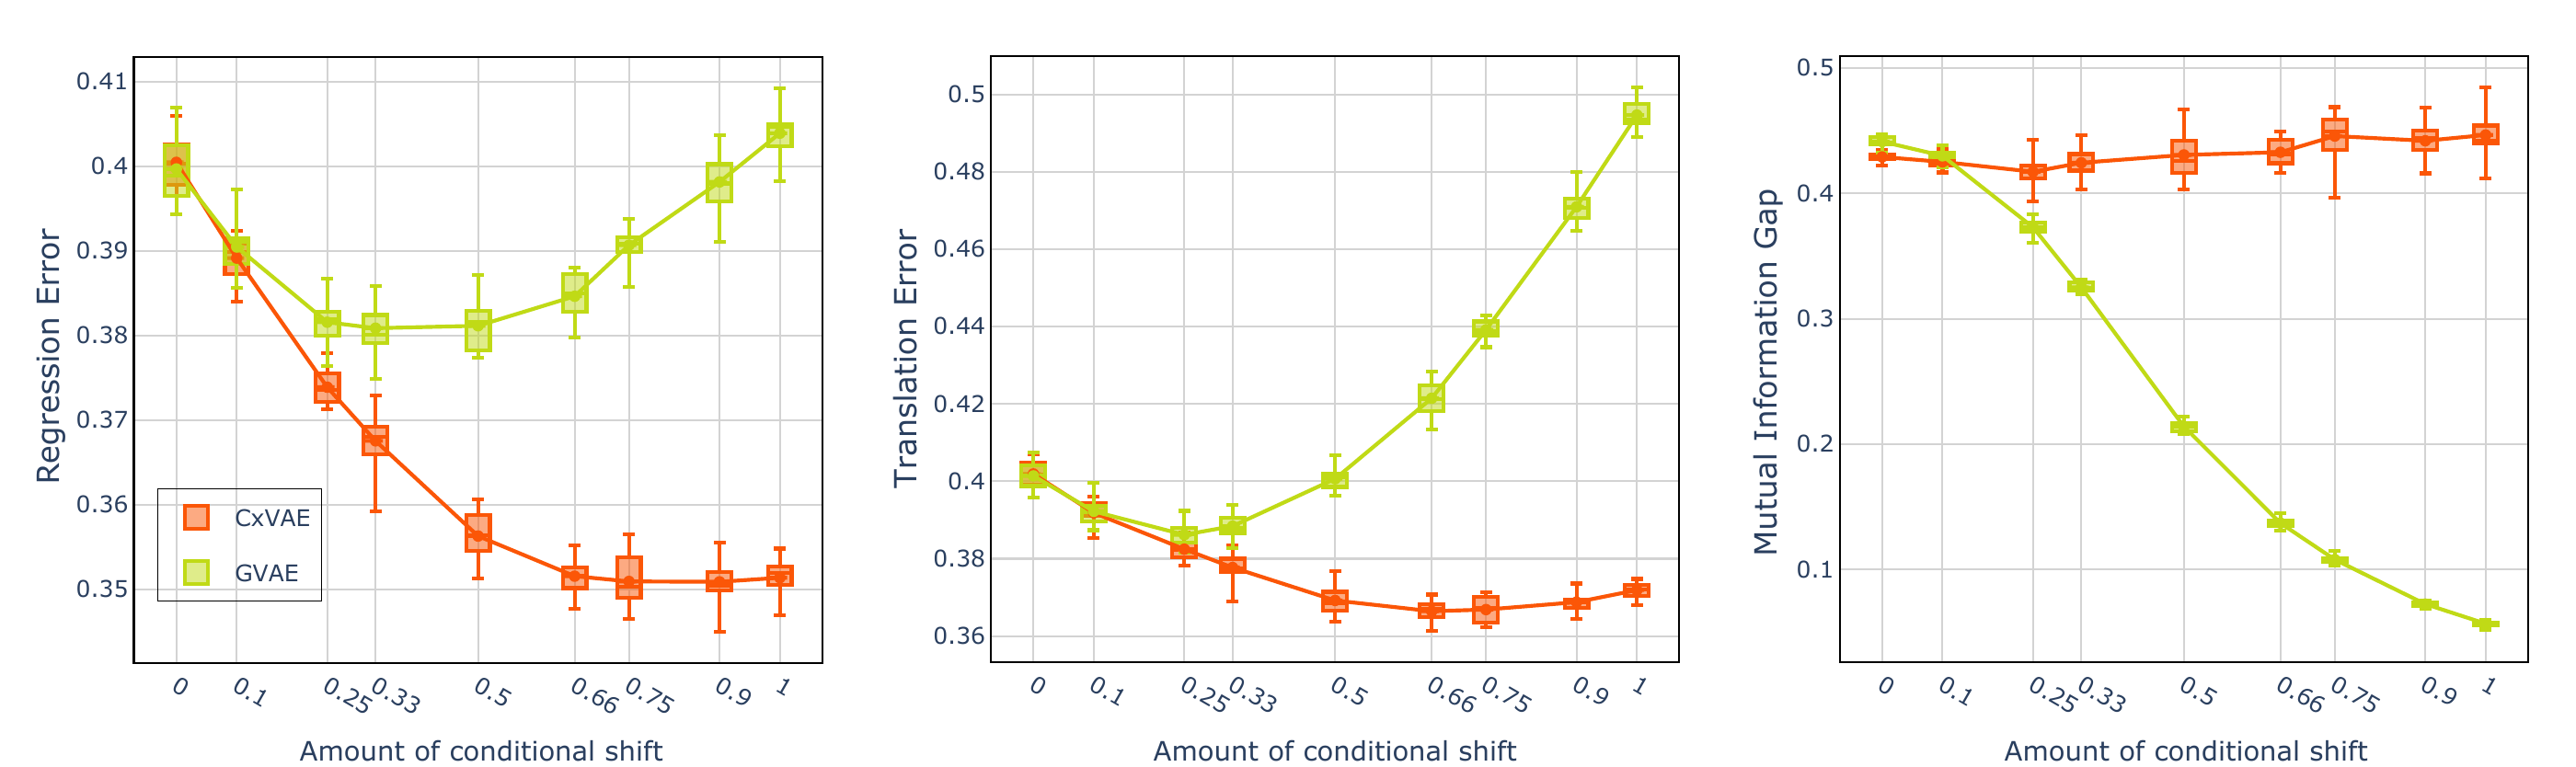
\includegraphics[width=\linewidth]{figures/xy_ratio.png}}
      \begin{center}
      \caption{Conditional shift in the dataset causes the relative performance gain of our CxVAE over the GVAE. We show performance on datasets generated with different values of the $\lambda$ hyper-parameter, controlling the amount of conditional shift. For low values of $\lambda$ the conditional density of student aptitude given a score changed very little from one group to another, and so CxVAE and GVAE perform equally well. However, as $\lambda$ increases, the GVAE fails to disentangle.}
      \label{fig:xy}
      \end{center}
      \vskip -0.0in
\end{figure*}

% \crit{[Explain why these metrics are legitimate. How do we know that they are not cherry-picked?]}

% We compare the models with respect to 3 different criteria: (a) How well do the content variables $\mathbf{c}$ predict the target variables $\mathbf{y}$? (b) How disentangled are the representations inferred by the encoder? (c) How well can the model answer the counterfactual question: ``What colour would appear if this object were lit by a different spotlight?'' We assess each criterion with a different evaluation metric.

\paragraph{Target Variable Regression.} After inferring the content variables, $\myrv{z}$, for the entire testing set, we use half of them as training inputs for a model to predict the ground-truth content variable, $\myrv{z}^{*}$. We use the other half to evaluate this predictor by taking the average mean-squared error between the prediction and the ground-truth content. This error will be our first measure of disentanglement. It reflects how much information about the ground-truth content is contained in the inferred content.

\paragraph{Mutual Information Gap.} We use the Mutual Information Gap \citep{chen2018isolating} to measure the quality of the disentanglement. We measure empirically the amount of mutual information between the inferred latent variables, $\myrv{w}$ and $\myrv{z}$, and the ground-truth style factor, $\myrv{w}^{*}$. Consequently, the goal is to have maximal mutual information between the inferred style variable, $\myrv{w}$, and the ground-truth style variable, $\myrv{w}^{*}$, and minimal mutual information between the inferred content variables, $\myrv{z}$, and the ground-truth style variable, $\myrv{w}^{*}$. The gap between the two (normalised with the entropy of the ground-truth factors) is the metric of disentanglement $\mathrm{MIG} = \frac{1}{H(\myrv{w}^{*})} (I(\myrv{w}; \myrv{w}^{*}) - I(\myrv{z}; \myrv{z}^{*}))$. 

Since, for both datasets, the data-generating process is known, the mutual information between the inferred style variable and the ground-truth style variable $I(\myrv{w}; \myrv{w}^{*})$ is straightforward to implement by following the approach from \citet{chen2018isolating}. We measure only the mutual information between the ground-truth group factor, $\myrv{w}^{*}$, and the latent variables because, as pointed out by \citet{nemethAdversarialDisentanglementGrouped2020}, the common failure case we are trying to guard against in style-content disentanglement is that the content variable, $\myrv{z}$, might learn information belonging to the ground-truth style factor $\myrv{w}^{*}$.

\paragraph{Translation Between Styles.} We measure how well the learned representations can answer the question ``What would the score of student $k$ from school $i$ have been if they had attended the \textit{typical} school (i.e., the school with scores distributed according to $\mathrm{N} (0, \mymatrix{i}_2)$)?''. This problem, also known as translation, is a commonly used downstream task for disentangled representations \citep{tenenbaum2000separating}. We translate the score of student $k$ to the typical school and then take the mean squared error against the ground-truth translation, which is generated when the data is generated using the ground-truth generative factors. 

% For our dataset, the correct translation corresponds to the Earth-Mover distance between the multivariate normal densitys of scores in each school \citep{knottOptimalMappingdensitys1984}. \crit{[Cryptic. There is a ground-truth, why do we need correct translations?]}

% \todo{\paragraph{How do we know what ground-truth translation should look like?} What is the point of the translation metric if it cannot be evaluated on real data? The authors say "Our model preserves the relative positions of the scores" in figure 2. It this something we desire naturally or something that comes out of an assumption? How can we guarantee relative positions of the features when translating without restrictions on q? What the desiderata for disentanglement here without stating the method? How should one evaluate them?}

In order to obtain the translation, we first infer the content variable of student $k$ from school $i$ and the style variable of the typical school. We then feed the two variables to the decoder. For evaluation, we translate all the scores from each school $n$ and then measure the distance between the predicted translation and the ground-truth translation. We compute the total error as an average over all the translation errors.

Translation is a well-established downstream task for evaluating disentanglement \citep{tenenbaum2000separating}. We can also use translation as an additional qualitative comparison between CxVAE and other group disentanglement methods, which can be seen in Figure~\ref{fig:trans}.

% In the case of the \texttt{TestScores} dataset, translation corresponds to the counterfactual question ``What score would student $k$ from school $A$ have obtained if they had attended the \textit{typical school} (i.e., a school whose scores are distributed according to $\mathrm{N}(0,\mymatrix{i}_2)$)?'' \crit{[This sentence seems out of place.]}

\section{Results}
\label{sec:results}

\begin{table}[t]
\vskip -0.0in
\caption{Our CxVAE model outperforms existing methods at disentanglement on the \texttt{Shift3DIdent} and \texttt{TestScores} datasets. The competing models are: GVAE \citep{hosoyaGroupbasedLearningDisentangled2019}, AdaGVAE \citep{locatelloWeaklySupervisedDisentanglementCompromises2020}, and COCO-FUNIT \citep{saitoCOCOFUNITFewShotUnsupervised2020}. The improvement in scores brought by our model is greater than the 95\% confidence interval around each score. Confidence intervals are computed by resampling train-test splits, weight initialisations and sampling seeds. All results are shown multiplied by 100.}
\label{table:results}
\begin{center}
\begin{tabularx}{\columnwidth}{lYYYYYY}
\toprule
& \multicolumn{3}{c}{\bf \texttt{Shift3DIdent}} & \multicolumn{3}{c}{\bf \texttt{TestScores}} \\ \midrule
{\sc Model}  & {\sc Rgrsn} $\downarrow$ & {\sc MIG} $\uparrow$ & {\sc Trnsl} $\downarrow$ & {\sc Rgrsn} $\downarrow$ & {\sc MIG} $\uparrow$ & {\sc Trnsl} $\downarrow$
\\ \midrule
GVAE & 8 $\pm$ 2 & 9 $\pm$ 6 & 23 $\pm$ 18 & 41 $\pm$ 1 & 4 $\pm$ 2 & 49 $\pm$ 1 \\
AdaGVAE & 9 $\pm$ 5 & 39 $\pm$ 11 & 15 $\pm$ 5 & 41 $\pm$ 1 & 5 $\pm$ 2 & 49 $\pm$ 1\\ 
CFUNIT & \textbf{5} $\pm$ 1 & 13 $\pm$ 4 & 13 $\pm$ 6 & 40 $\pm$ 2 & 4 $\pm$ 1 & 49 $\pm$ 2 \\
\textbf{CxVAE} & \textbf{5} $\pm$ 3 & \textbf{72} $\pm$ 6 & \textbf{8} $\pm$ 5 & \textbf{35} $\pm$ 2 & \textbf{44} $\pm$ 8 & \textbf{37} $\pm$ 2\\
\bottomrule
\end{tabularx}
\end{center}
\vskip -0in
\end{table}

We show that our CxVAE is able to disentangle style and content in a setting where conditional shift produces ambiguous observations. The results in Table~\ref{table:results} show that our model, CxVAE, produces representations that disentangle between spotlight colour and object colour much more than a representative selection of existing models: GVAE~\citep{hosoyaGroupbasedLearningDisentangled2019,bouchacourt2017multi}, AdaGVAE~\citep{locatelloWeaklySupervisedDisentanglementCompromises2020}, and COCO-FUNIT~\citep{saitoCOCOFUNITFewShotUnsupervised2020}. Our model's MIG score is much higher than the one produced by competing models and the performance gap is greater than the 95\% confidence interval for any one of these models.

Our CxVAE produces considerable improvements over the competing methods in terms of fitting the holdout set, disentangled representations, translation accuracy, and predicting the generative factors (Table~\ref{table:results}). While the scores of the existing methods cluster together, the gap between them and CxVAE is larger than the 95\% confidence interval of any method.

\section{Conditional Shift Causes the Gap in Performance}
\label{sec:xy}

By modifying the data-generating process of the \texttt{TestScores} dataset, we show that conditional shift explains the increased performance of CxVAE. We insert a hyper-parameter $\lambda$ to control the strength of the conditional shift; $\lambda=1$ means the conditional shift stays the same as in the previous experiment, while $\lambda=0$ means there is no conditional shift. 

Consider the case where the maths score only depends on the school and the reading score only depends on the student. In this situation, the two generative factors can be easily disentangled since you can infer the student aptitude from the reading score and the school profile from the maths score. We use this as an extreme case of lack of conditional shift and insert a hyper-parameter $\lambda$ in our data-generating process that will continuously move between this case and the original case. Our modified data-generating process is:
\[
      \forall i \in \{1,\dots,\mycnt{n}\}, \quad \beta^i \sim \mathrm{N}(0,\mymatrix{i}_2), \quad \gamma^i \sim \mathrm{N}(0,\mymatrix{i}_2), \quad \forall k \in \left\{1,\dots,\mycnt{m}^i\right\}, \quad \alpha^i_k \sim \mathrm{N}(0,\mymatrix{i}_2),
\]
\[
      \myvect{x}^{i}_k = \begin{bmatrix} \lambda \\ 1 \end{bmatrix} \odot \beta^i + \begin{bmatrix} 1 \\ \lambda \end{bmatrix} \odot \alpha^i_k \odot \left(\gamma^i \blacklozenge \begin{bmatrix} \lambda \\ 1 \end{bmatrix} \right) + \epsilon^i_k, \quad \epsilon^i_k \sim \mathrm{N}(0,\, 0.1 \cdot \mymatrix{i}_2),
\]
where $\blacklozenge$ denotes the elementwise power operation. 

This data-generating process has no conditional shift when $\lambda=0$ because each ground-truth factor controls a separate component of the data. Inferring the student aptitude requires only the reading score and the school characteristics can be ignored. When $\lambda=1$, the problem exhibits conditional shift in exactly the same way as before. 

% \crit{[This thought experiment belongs much earlier. Leave the results here, but place the problem earlier.]}

We hypothesise that the conditional shift causes the performance gap between CxVAE and other group disentanglement methods. If our hypothesis is correct, then the gap should decrease as $\lambda$ approaches  The measurements displayed in Figure \ref{fig:xy} confirm our expectations. For low values of $\lambda$ the performance of our CxVAE is evenly matched to the GVAE.  As $\lambda$ increases, CxVAE metrics remain stable while GVAE performance decreases substantially.  It is clear that the degree of confounding in the dataset explains the performance gain that we see in CxVAE. 

\section{Conclusions}
\label{sec:conclusion}

In this work, we show empirically that conditioning the content encoder on the style variable produces style-content disentangled representations on datasets with conditional shift. We also show that the strength of the conditional shift effect in the data-generating process determines the amount of improvement that our model brings over other group disentanglement methods. Our evaluation is run on two important downstream tasks for style-content disentanglement: One is the problem of inferring student aptitudes from test scores grouped by school, and another is identifying the colours of objects viewed under different lighting conditions.

% The main limitation of our work is that we perform evaluation on a synthetic dataset of student scores rather than real data. Although this is a justifiable choice with respect to evaluation (it gives us access to the ground-truth values of the latent variables), future work should focus on evaluating on real-world datasets with conditional shift, such as user-item ratings \citep{Koren2009MatrixFT}.

% \crit{[1) The reviewers thought that the method is not well motivated. Why is conditioning on the group variable necessary? i.e. Why does it help? 2) What are the assumptions of conditional shift and what is the space of problems? 3) Implementation details 4) Synthetic data.]}
      

\biblio

\end{document}
